\documentclass[11pt,letterpaper]{article}
\usepackage[margin=1in]{geometry}
\usepackage[T1]{fontenc}
\usepackage{newtxtext,newtxmath}
\usepackage{microtype}
\usepackage{graphicx}
\usepackage[font=small,labelfont=bf,labelsep=period]{caption}
\usepackage[authoryear,round]{natbib}
\usepackage[hidelinks]{hyperref}

\hypersetup{
  pdftitle={Lateral OFC represents reward identity during conditioning},
  pdfsubject={Proposed Results and Methods text for PI review}
}
\setlength{\parindent}{0pt}
\setlength{\parskip}{0.8\baselineskip}
\pagestyle{plain}

\begin{document}

{\small\sffamily Draft for PI review \hfill November 12, 2026\par}
\vspace{0.4\baselineskip}
{\Large\bfseries Lateral OFC represents reward identity during conditioning\par}
\vspace{0.4\baselineskip}

\section*{Results}

The preferential representation of preconditioned outcomes in lateral OFC may reflect the prioritization of inferred outcome identities when both cue classes share limited representational resources. We therefore asked whether directly conditioned cues would evoke odor-related representations during conditioning, when only conditioned cues were presented and participants explicitly reported which odor would follow each cue (Fig.~\ref{fig-conditioning-identity}A). Using the same independently defined lateral and medial OFC regions, we tested whether cues predicting the same food odor evoked more similar neural patterns than cues predicting different odors. RSA used single-trial activity estimates spanning the combined cue and prediction period (0--5\,s), pooled correct trials across all available conditioning runs ($n = 29$), and excluded clean-air trials. Pattern comparisons were restricted to presentations from different runs.

Neural patterns in lateral OFC showed a small positive correspondence with the odor-identity model (mean Spearman $\rho = 0.0131$, $t(28) = 2.01$, $p = 0.027$), whereas the corresponding effect was not significant in medial OFC (mean Spearman $\rho = 0.0068$, $t(28) = 1.20$, $p = 0.120$; both $p$ values one-sided and uncorrected; Fig.~\ref{fig-conditioning-identity}B, left).

To test whether conditioning cues also evoked patterns shared with experienced odors, we trained the same cross-task decoder on responses to the two food odors in the independent passive localizer and applied it to conditioning cue patterns from an early cue window (0--2\,s; EARLY) and the combined cue and prediction window (0--5\,s; EXT5s). In lateral OFC, balanced accuracy exceeded 50\% chance for EARLY (52.12\%, $t(28) = 1.83$, $p = 0.039$; Fig.~\ref{fig-conditioning-identity}B, right). Accuracy was also numerically above chance for EXT5s, although this effect did not reach significance (51.87\%, $t(28) = 1.45$, $p = 0.079$). Decoding was not significantly above chance in medial OFC for either window (EARLY, 49.25\%, $p = 0.715$; EXT5s, 50.05\%, $p = 0.484$; all decoding $p$ values one-sided and uncorrected). Together, these analyses provide suggestive evidence of odor-related information in lateral OFC during explicit prediction of directly associated outcomes, consistent with previous findings of identity-specific reward representations in this region \citep{howard2015identity,howard2017identity}.

\renewcommand{\thefigure}{X}
\begin{figure}[p]
\centering
\makebox[\linewidth][c]{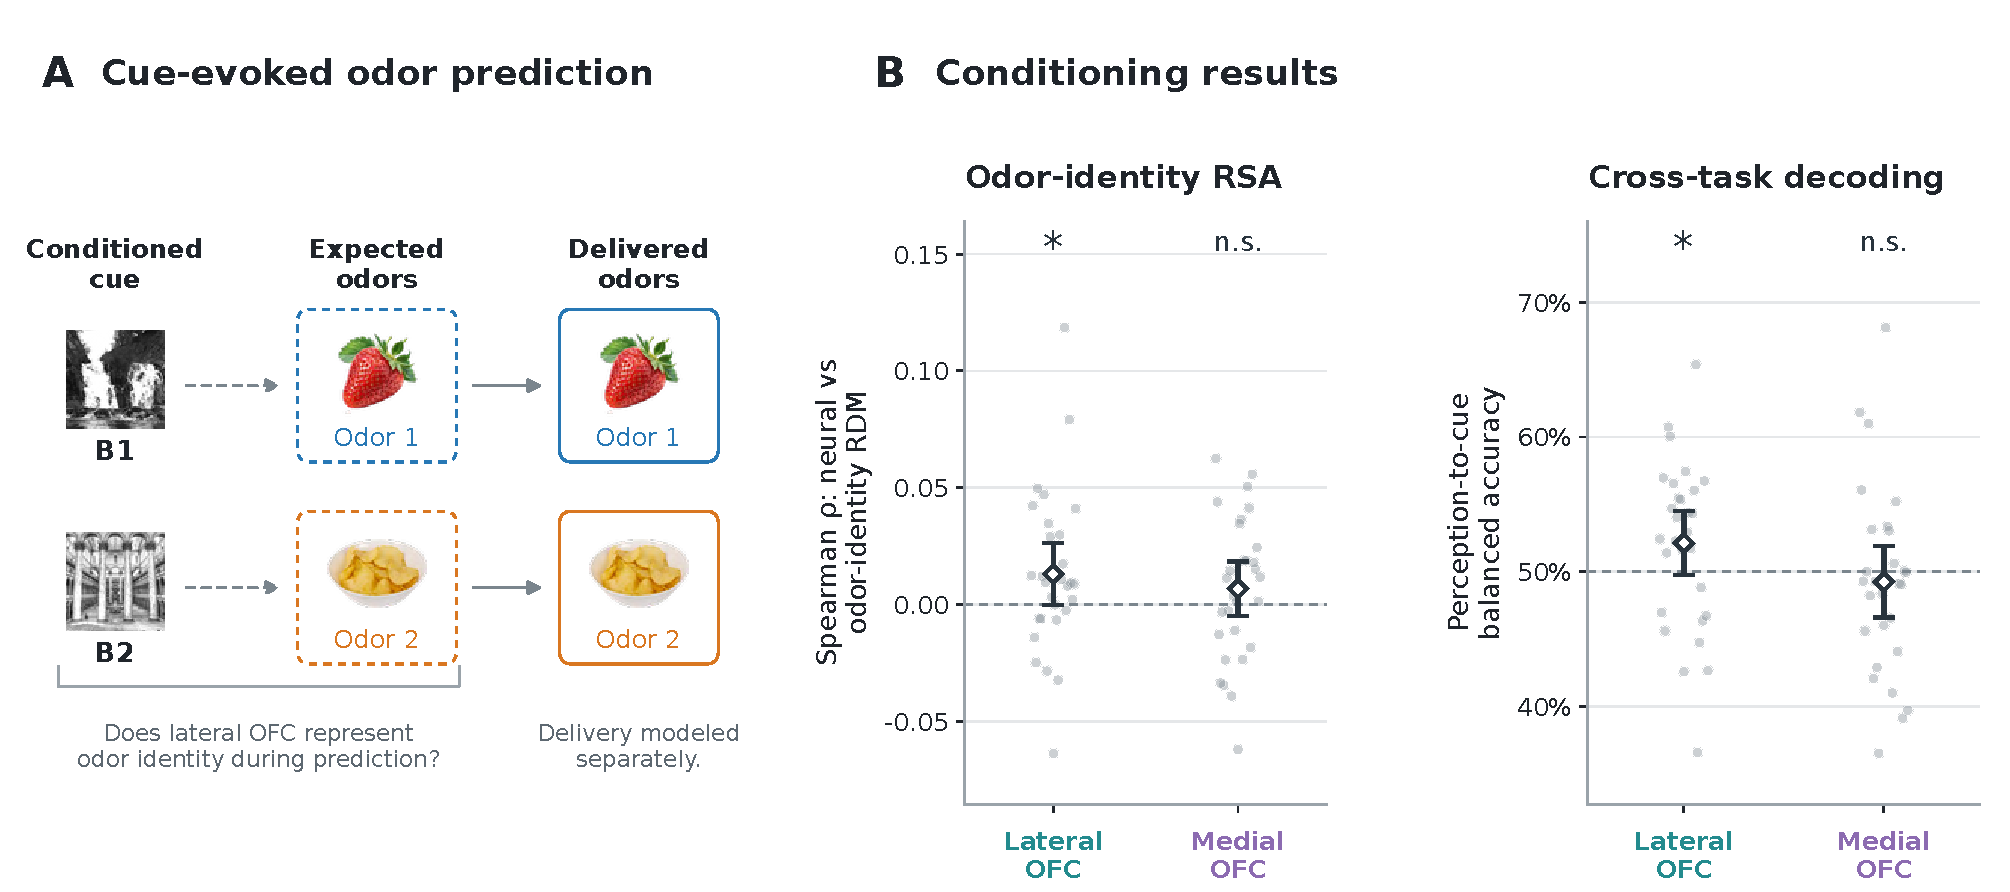
\includegraphics[width=\dimexpr\linewidth+1in\relax]{../../fig/figx.pdf}}
\caption{
\textbf{Lateral OFC represents reward identity during conditioning.}
\textbf{A. Cue-evoked odor prediction during conditioning.} Illustrative food-odor trials show directly conditioned cues (B1/B2), prediction of their associated odors, and subsequent odor delivery. Dashed arrows link cues to their expected odors; solid arrows indicate subsequent odor delivery. Dashed boxes depict expected outcomes, not odor images displayed during the task; solid boxes indicate delivered odors. The intervening delay is omitted. The bracket groups the cue and prediction stages targeted by the analyses. Cue and odor assignments follow the illustrative mapping in Figure~1 and were counterbalanced across participants. Odor-delivery events for both food odors and clean air were included as one pooled nuisance regressor in the single-trial cue GLMs, modeling delivery separately from cue-evoked responses.
\textbf{B. Conditioning results.} Left plot: odor-identity RSA. Spearman correlations between neural and expected odor-identity RDMs were computed from single-trial estimates spanning the cue and prediction period (0--5\,s after cue onset; EXT5s), retaining only comparisons between presentations from different runs. Right plot: cross-task decoding. A linear support vector machine trained to distinguish the two food odors in the independent passive localizer was tested on early conditioning cue estimates (0--2\,s; EARLY). Balanced accuracy averages classification accuracy across the two odor identities. Both analyses used correct food-odor trials pooled across all available conditioning runs in the same participants ($n = 29$; 28 contributed three runs and one contributed runs 1--2). The independently defined bilateral OFC regions are the same as in Figure~3. Points represent individual participants, and open diamonds show means with $t$-based 95\% confidence intervals. Dashed lines indicate zero RSA correlation (left) and 50\% chance accuracy (right). Asterisks denote uncorrected $p < 0.05$ from one-sided one-sample $t$-tests against these respective baselines; n.s., not significant.
}
\label{fig-conditioning-identity}
\end{figure}

\clearpage
\section*{Methods}

Conditioning single-trial GLMs used the same preprocessed images and nuisance regressors as the probe models. Each least-squares-separate model contained a target-cue regressor and a second regressor pooling all other cue presentations, spanning either the first 2\,s (EARLY) or the combined cue and prediction period (5\,s; EXT5s). EARLY models additionally included a pooled prediction regressor (2--5\,s after cue onset). Both models included delay (5--7\,s), odor delivery (7--9\,s), zero-duration button presses at the recorded response times, and fixation replacing delay and delivery on missed-response trials (4\,s). Delivery events for both food odors and clean air were pooled into one regressor and included on all responded trials, including incorrect predictions. All cue presentations were modeled; correct-trial filtering was applied subsequently.

RSA and cross-task decoding used the same bilateral OFC regions as the probe analyses. Only correct food-odor trials with recorded responses and finite positive response times were retained, pooling all available conditioning runs. Two additional participants were excluded for sparse correct trials and severe OFC coverage loss, leaving 29 participants; 28 contributed three runs and one contributed runs 1--2 because the third scan was interrupted. RSA used EXT5s estimates and the probe-analysis procedures, with participant-level coefficients assessed against zero. Cross-task decoding followed the probe-analysis procedure, training a classifier on passive odor-localizer patterns and applying it to both conditioning windows without further fitting. EARLY and EXT5s used matched trials and a common set of voxels finite across training and testing; voxel responses were z-scored separately within each task, window, and run. Balanced accuracy averaged recall across the two food odors and was assessed against 50\% chance. Both analyses used one-sided one-sample $t$-tests with uncorrected $p$ values.

{\small
\bibliographystyle{plainnat}
\bibliography{../main/sn-bibliography}
}

\end{document}
